\subsection{Jacobi Matrix}
Die Jacobimatrix (oder Funktionalmatrix) einer Funktion $F$ besteht aus den ersten partiellen Ableitungen von allen Komponenten nach allen Variabeln. Also aus den Gradienten von jeder Komponente. Sei $F: \R^n \to \R^m$, dann gilt:
\begin{align*}
	JF = DF =
	\left(\begin{array}{cccc}
		\vspace{0.2cm}\frac{\partial F_1}{\partial x_1} & \frac{\partial F_1}{\partial x_2} & \ldots & \frac{\partial F_1}{\partial x_n}\\
		\vspace{0.1cm}\frac{\partial F_2}{\partial x_1} & \frac{\partial F_2}{\partial x_2} & \ldots & \frac{\partial F_2}{\partial x_n}\\
		\vspace{0.05cm}\vdots & \vdots & & \vdots\\
		\frac{\partial F_m}{\partial x_1} & \frac{\partial F_m}{\partial x_2} & \ldots & \frac{\partial F_m}{\partial x_n}
	\end{array}\right)
	=
	\left(\begin{array}{c}
		\vspace{0.2cm} - \nabla F_1 -\\
		\vspace{0.1cm} - \nabla F_2 -\\
		\vspace{0.05cm}\vdots\\
		- \nabla F_m -
	\end{array}\right)
\end{align*}

\subsubsection{Jacobi Determinante}
Ist einfach die Determinante der Jacobimatrix. Will man das Integral über einen Bereich ausrechnen, welcher in einem anderen Koordinatensystem einfacher ist, dann muss zusätzlich zur Koordinatentransformation, das Integral mit der Jacobideterminante für dieses neue Koordinatensystem multipliziert werden!\\
Bsp. Für die Polarkoordinaten ist die Jacobi Determinante:
\[
	F = 
	\left(\begin{array}{c}
		r \cdot \cos(\phi) \\
		r \cdot \sin(\phi)
	\end{array}\right)
	\Rightarrow
	|JF| = 
	\left|\begin{array}{cc}
		\cos(\phi) & -r \cdot \sin(\phi)\\
		\sin(\phi) & r \cdot \cos(\phi)\\
	\end{array}\right|
	= r
\]
\section{Koordinatensysteme}
\vspace{-0.1cm}\subsection{Koordinaten im $\R^2$}
\textbf{Polarkoordinaten $(r, \phi)$:}\\
\begin{align*}
	x &= r \cdot \cos(\phi) &  r &= \sqrt{x^2 + y^2} & 0 &\leq r \leq \infty\\
	y &= r \cdot \sin(\phi) &  \phi &= arg(x, y) & 0 &\leq \phi < 2\pi
\end{align*}

\begin{minipage}{0.6\columnwidth}
	Jacobideterminante: $r$\\
	Integralsubstitution: $dx \, dy \to r \, dr \, d\phi$
\end{minipage}
\begin{minipage}{0.39\columnwidth}
	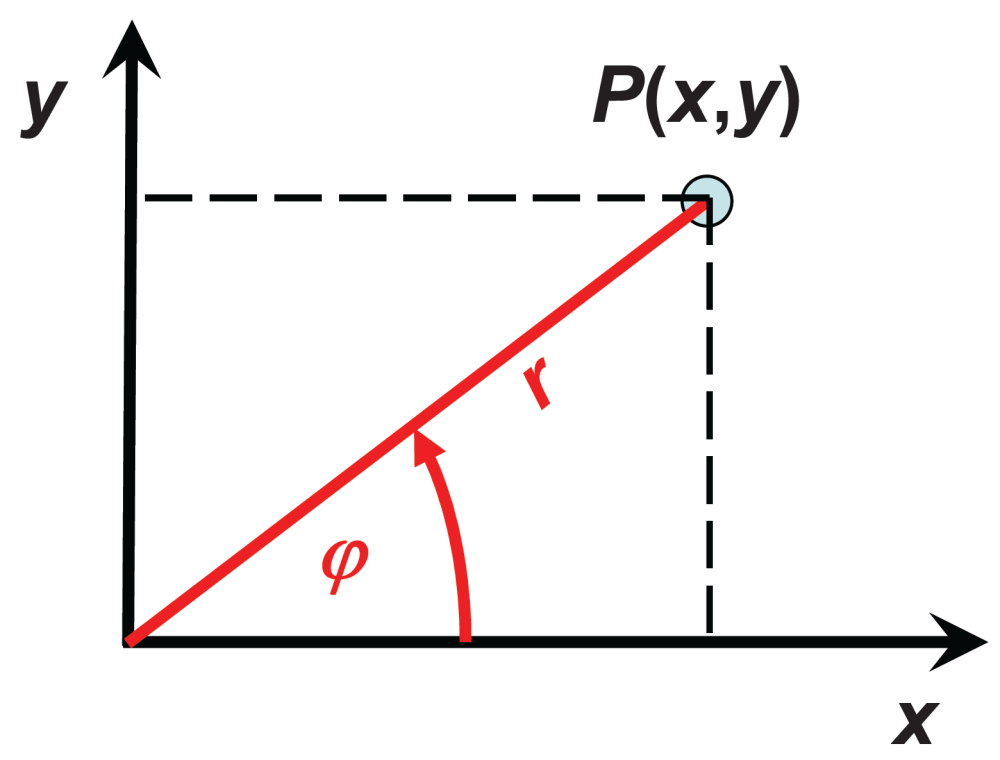
\includegraphics[width=\columnwidth]{polar_coordinate}
\end{minipage}

\vspace{-0.3cm}\subsection{Koordinaten im $\R^3$}
\textbf{Kugelkoordinaten I $(r, \vartheta, \phi)$:}\\
\begin{align*}
	x &= r \cdot \sin(\vartheta) \cdot \cos(\phi) & r &= \sqrt{x^2 + y^2 + z^2} & 0 &\leq r \leq \infty\\
	y &= r \cdot \sin(\vartheta) \cdot \sin(\phi) & \phi &= arg(x, y) & 0 &\leq \phi < 2\pi\\
	z &= r \cdot \cos(\vartheta) & \vartheta &= \arccos({\small \frac{z}{\sqrt{x^2 + y^2 + z^2}}}) & 0 &\leq \vartheta \leq \pi
\end{align*}
Jacobideterminante: $r^2 \cdot \sin(\vartheta)$\\
Integralsubstitution: $dx \, dy\, dz \to r^2 \cdot \sin(\vartheta) \, dr \, d\phi \, d\vartheta$

\textbf{Kugelkoordinaten II $(r, \vartheta, \phi)$:}\\
\begin{align*}
	x &= r \cdot \cos(\vartheta) \cdot \cos(\phi) & r &= \sqrt{x^2 + y^2 + z^2} & 0 &\leq r \leq \infty\\
	y &= r \cdot \cos(\vartheta) \cdot \sin(\phi) & \phi &= arg(x, y) & 0 &\leq \phi < 2\pi\\
	z &= r \cdot \sin(\vartheta) & \vartheta &= \arcsin({\small \frac{z}{\sqrt{x^2 + y^2 + z^2}}}) &\hspace{-0.15cm}-\frac{\pi}{2} &\leq \vartheta \leq \frac{\pi}{2}
\end{align*}
Jacobideterminante = $r^2 \cdot \cos(\vartheta)$\\
Integralsubstitution: $dx \, dy\, dz \to r^2 \cdot \cos(\vartheta) \, dr \, d\phi \, d\vartheta$

\begin{minipage}{0.5\columnwidth}
	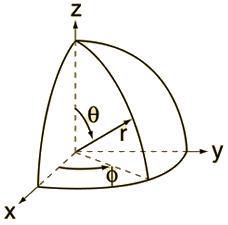
\includegraphics[width=\columnwidth]{kugel_coordinates_I.png}\\
	Kugelkoordinaten I
\end{minipage}
\begin{minipage}{0.5\columnwidth}
	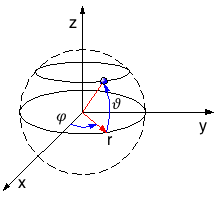
\includegraphics[width=\columnwidth]{kugel_coordinates_II.png}\\
	Kugelkoordinaten II
\end{minipage}

\textbf{Zylinderkoordinaten $(r, \phi, z)$:}\\
\begin{align*}
	x &= r \cdot \cos(\phi) &  r &= \sqrt{x^2 + y^2} & 0 &\leq r \leq \infty\\
	y &= r \cdot \sin(\phi) &  \phi &= arg(x, y) & 0 &\leq \phi < 2\pi\\
	z &= z & z &= z & -\infty & \leq z \leq \infty
\end{align*}
\begin{minipage}{0.68\columnwidth}
	Jacobideterminante: $r$\\
	Integralsubstitution: $dx \, dy \, dz \to r \, dr \, d\phi \, dz$
\end{minipage}
\begin{minipage}{0.31\columnwidth}
	\hspace{-0.3cm}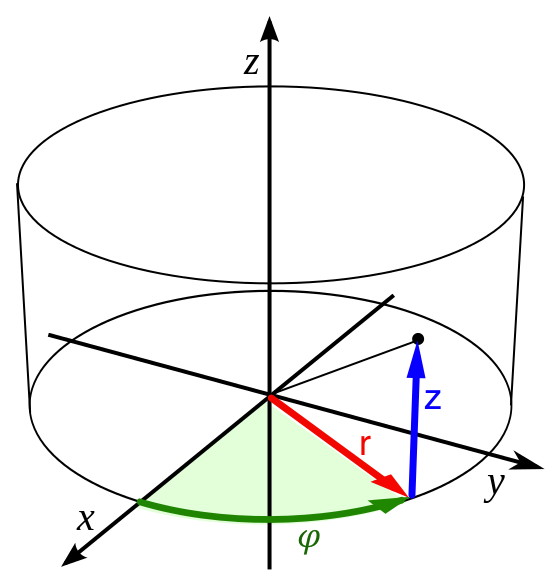
\includegraphics[width=1.1\columnwidth]{cylindrical_coordinates}
\end{minipage}

\textbf{arg(x, y) für $0 \leq \phi < 2\pi $}\\
$arg(x, y) =
\begin{cases}
	\arctan(\frac{y}{x})				& x > 0 \gtext{und} y \geq 0 \\
	\arctan(\frac{y}{x}) + 2\pi			& x > 0 \gtext{und} y < 0 \\
	\arctan(\frac{y}{x}) + \pi			& x < 0\\
	\frac{\pi}{2}						& x = 0 \gtext{und} y > 0\\
	\frac{3\pi}{2}						& x = 0 \gtext{und} y < 0\\
	0 									& x = 0 \gtext{und} y = 0
\end{cases}
$

\textbf{arg(x, y) für $-\pi < \phi \leq \pi$}\\
$arg(x, y) =
\begin{cases}
	\arctan(\frac{y}{x})				& x > 0 \\
	\arctan(\frac{y}{x}) + \pi			& x < 0 \gtext{und} y \geq 0 \\
	\arctan(\frac{y}{x}) - \pi			& x < 0 \gtext{und} y < 0 \\
	\frac{\pi}{2}						& x = 0 \gtext{und} y > 0\\
	-\frac{\pi}{2}						& x = 0 \gtext{und} y < 0\\
	0 									& x = 0 \gtext{und} y = 0
\end{cases}
$\\
\begin{minipage}{0.68\columnwidth}
	\textbf{Beispiel:}\\
	Berechne die Fläche des Halbkreisrings\\
	$R: 1 \leq x^2 + y^2 \leq 4$ und $y \geq 0$:
\end{minipage}
\begin{minipage}{0.31\columnwidth}
	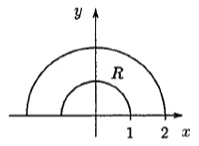
\includegraphics[width=\columnwidth]{example_polar_coordinates}
\end{minipage}

Die Fläche lässt sich mit Polarkoordinaten besonders einfach ausrechnen. Die Parametrisierung für $r$ und $\phi$ lässt sich leicht aus der Grafik ablesen:
\begin{align*}
	x &= r \, \cos(\phi)	&& 1 \leq r \leq 2 \\
	y &= r \, \sin(\phi)	&& 0 \leq \phi \leq \pi
\end{align*}
Das Flächenintegral ist somit:
\begin{align*}
	R = \int_R dx \, dy = \int_R r \, dr \, d\phi = \int_0^{\pi} \int_1^2 r \, dr \, d\phi = \pi \left[\frac{r^2}{2}\right]_1^2 = \uuline{\frac{3}{2} \pi}
\end{align*}


\newpage
\subsection{Divergenzsatz im $\R^2$}
\begin{minipage}{0.68\columnwidth}
	Sei $G \subset \R^2$ eine Fläche mit Randkurve $C$ und äusserem Normalenvektor $\vec{n}$. $F$ sei ein Vektorfeld. Dann gilt:
	\[
		\int_{C} F \cdot \vec{n} \, ds = \int\int_G \operatorname{div} F \, dx \, dy
	\]
\end{minipage}
\begin{minipage}{0.31\columnwidth}
	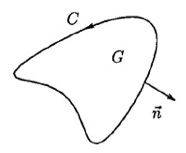
\includegraphics[width=\columnwidth]{divergenzsatz_r2}
\end{minipage}
Dh: Der Fluss des Vektorfelds durch die Randkurve $C$, ist gleich dem Integral der Quellenstärke im Innern der Fläche $G$!\\

\begin{minipage}{0.75\columnwidth}
	\textbf{Beispiel:}\\
	Berechne den Fluss von 
	$F(x, y) = 
	\left(
	\begin{array}{c}
		x^3\\
		0 
	\end{array}\right)$
	durch den Rand des Kreises mit Radius 2:
\end{minipage}
\begin{minipage}{0.24\columnwidth}
	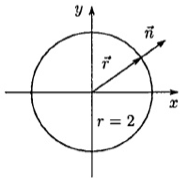
\includegraphics[width=\columnwidth]{example_divergence_theorem}
\end{minipage}
Dazu verwenden wir den Divergenzsatz (Satz von Gauss) und nehmen Polarkoordinaten:
\begin{align*}
	\operatorname{div} F &= 3x^2 && 0 \leq r \leq 2 \gtext{und} 0 \leq \phi \leq 2\pi \\
	\int_{C} F \cdot \vec{n} \, ds &= 
	\int\int_G 3x^2 \, dx \, dy &&= 
	\int_0^{2\pi} \int_0^2 3 r^2 \cos(\phi)^2 \, r \; dr \, d\phi \\
	& &&= 3 \left[ \frac{r^4}{4} \right]_0^2 \cdot \left[ \frac{\phi}{2} + \frac{1}{4} \sin(2\phi) \right]_0^{2\pi} \\
	& &&= 3 \cdot 4 \cdot \pi = 12 \pi
\end{align*}
 
\subsection{Divergenzsatz im $\R^3$}
\begin{minipage}{0.68\columnwidth}
	Sei V $\subset \R^3$ ein Gebiet mit Randfläche (Oberfläche) S = $\partial V$ und äusserem Flächennormalenvektor $\vec{n}$. $F$ sei ein Vektorfeld. Dann ist:
	\[
		\int \int_S F \cdot \vec{n} \; dS = \int \int \int_V \operatorname{div} F \; dx \, dy \, dz
	\]	
\end{minipage}
\begin{minipage}{0.31\columnwidth}
	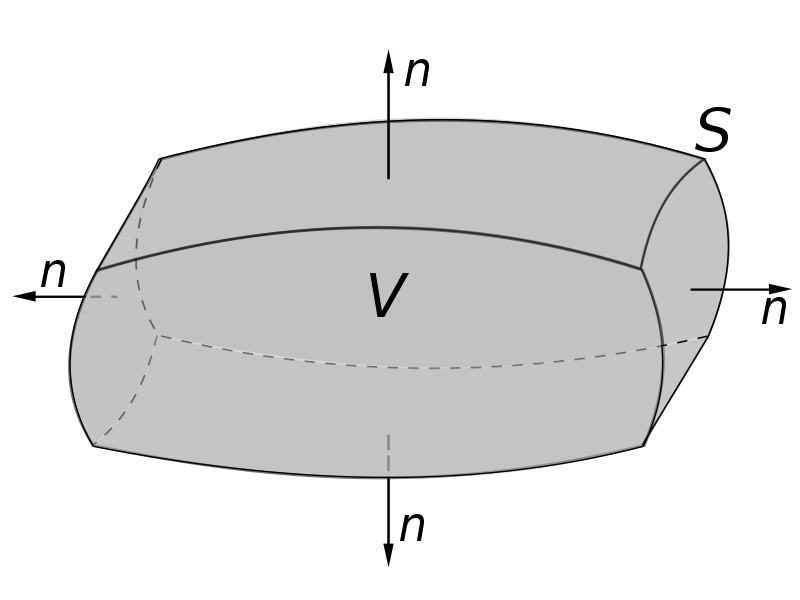
\includegraphics[width=\columnwidth]{divergence_theorem_r3}
\end{minipage}
Dh: Der Fluss des Vektorfelds durch die Randfläche des Gebiets ist gleich dem Integral der Quellenstärke im Innern!

\subsection{Massenschwerpunkt vs. Volumenschwerpunkt}
Ist der Körper homogen (besteht er also aus gleichem Material mit überall gleicher Dichte), so ist der Massenschwerpunkt gleich dem geometrischen Volumenschwerpunkt. Besteht der Körper jedoch aus Teilen mit verschiedener Dichte, kann der Massenschwerpunkt vom Volumenschwerpunkt abweichen!

\subsubsection{Volumenschwerpunkt}
Der Schwerpunkt eines beschränkten Körpers $K$ im dreidimensionalen Raum mit Volumen $V$ ist (im kartesischen Koordinatensystem) definiert als:
\[
	x_s = \frac{1}{V} \int_K x \, dV \gap y_s = \frac{1}{V} \int_K y \, dV \gap z_s = \frac{1}{V} \int_K z \, dV
\]
\[
	\text{mit } V = \int_K \; dV
\]
\textbf{Merke:} 
$\int_K$ steht für $\int_a^b \int_c^d \int_e^f$ und $dV$ für $dx \,dy \, dz$. Wenn also der Schwerpunkt für ein anderes Koordinatensystem ausgerechnet werden muss, muss man auch ein Integralsubstitution vornehmen (siehe Koordinatentransformation)!

\subsubsection{Massenschwerpunkt}
Der Schwerpunkt eines beschränkten Körpers $K$ im dreidimensionalen Raum mit Masse $M$, Volumen $V$ und Dichte $\rho$ ist (im kartesischen Koordinatensystem) definiert als:
\[
	x_s = \frac{1}{M} \int_K x \cdot \rho \, dV \gap 
	y_s = \frac{1}{M} \int_K y \cdot \rho \, dV \gap 
	z_s = \frac{1}{M} \int_K z \cdot \rho \, dV
\]
\[
	\text{mit } M = \int_K \rho \, dV = \int_a^b \int_c^d \int_e^f \rho \, dx \, dy \, dz
\]
\textbf{Merke:} $\rho = \frac{M}{V}$\\

\section{Weitere Beispiele}
\textbf{Bsp. Zwischenwertsatz}\\
Seien $c, d \in \R$ und $c < d$. Zeige mit Zwischenwertsatz, dass die nachfolgende Gleichung eine Lösung im Intervall $]c, d[$ hat.
\[
	\frac{2}{(x - c)^4} + \frac{5}{(x - d)^9} = 0
\]
Wir definieren $f(x) = \frac{2}{(x - c)^4} + \frac{5}{(x - d)^9}$\\
Gesucht ist also ein $x \in ]c, d[$, so dass die Gleichung erfüllbar ist! 
Dazu suchen wir zwei Punkte $x_1, x_2$ mit $c < x_1 < x_2 < d$ so dass $f(x_2) < 0 < f(x_1)$   (oder $f(x_1) < 0 < f(x_2)$).
\[
	\lim_{x \to c^{+}} \ucomment{+ \infty}{\frac{2}{(x - c)^4}} + \ucomment{const.}{\frac{5}{(x - d)^9}} = + \infty
\]
$\Rightarrow$ Wir finden also sicher ein $x_1$ mit $c < x_1 < \frac{c + d}{2}$ und $f(x) > 0$!
\[
	\lim_{x \to d^{-}} \ucomment{const.}{\frac{2}{(x - c)^4}} + \ucomment{- \infty}{\frac{5}{(x - d)^9}} = - \infty
\]
$\Rightarrow$ Wir finden also sicher ein $x_x$ mit $\frac{c + d}{2} < x_2 < d$ und $f(x) < 0$!

Da die Funktion stetig ist, und wir zwei Punkte $x_1 < x_2$ gefunden haben für die gilt $f(x_2) < 0 f(x_1)$ folgt aus dem Zwischenwertsatz, dass es ein $x \in ]c, d[$ geben muss sodass $f(x) = 0$!